\section{CPU Efficient Cracking}
\label{sec:cracking-algorithms}
Based on the outcome of our analysis in the previous section, we can
direct our efforts to the performance painpoints of the original
\emph{Cracking} implementation, starting with branch mispredictions.

\subsection*{Predication}
\label{sec:predication}
A common technique to address costs for branch mispredictions is
``predication''. The idea is to unconditionally write output but only
advance one of the output cursors by the value of the evaluation of
the predicate. This decouples the writing operation from the predicate
evaluation and, therefore, effectively eliminates the conditional
branch instructions at the costs of more write instructions. Since
these write instructions generally only operate in L1 cache, the
performance benefit for, e.g., selections, can be
significant~\cite{ross2004selection}.
\begin{figure}[h]
\subfloat[Consistent State]{
  \includegraphics[width=.9\columnwidth]{Figures/damon/PredicationPhase1}
\label{fig:predicated-consistent}
}

\subfloat[Compare \& Write Phase]{
  \includegraphics[width=.9\columnwidth]{Figures/damon/PredicationPhase2}
\label{fig:predicated-compare-and-write}
}

\subfloat[Advance Cursor Phase]{
  \includegraphics[width=.9\columnwidth]{Figures/damon/PredicationPhase3}
\label{fig:predicated-advance-cursor}
}

\subfloat[Backup Phase]{
  \includegraphics[width=.9\columnwidth]{Figures/damon/PredicationPhase4}
\label{fig:predicated-backup}
}
  \caption{Predicated Cracking}
  \label{fig:predicated-cracking}
\end{figure}


Unfortunately, not all algorithms are equally amenable to
optimization through predication: implementations of out-of-place
algorithms like selections can speculatively write to the output
buffer as long as they write to empty slots. In-place algorithms,
however, have to ensure that they do not overwrite any of the data
values. They, therefore have to create backup copies of values
that are speculatively overwritten. Naturally, deciding which value
to backup has to be branch-free as well.

To achieve this, we developed a branch-free cracking implementation
based on predication (illustrated in
Figure~\ref{fig:predicated-cracking}). The fundamental idea is to
create a backup copy of the value that is speculatively overwritten in
a ``backup'' slot (we term the slot containing the value that is
currently processed ``active''). Based on this idea, each iteration
goes through multiple phases with all (significant) operations within
a phase being independent. At the beginning of each iteration, the
to-be-cracked array is in a ``consistent'' state (see
Figure~\ref{fig:predicated-consistent}), i.e., each input value is
stored exactly once in the array\footnote{Note that this does not
  imply that there cannot be duplicate values in the input} and the
``active'' and ``backup'' slots contain the values at both cursors.
In the \emph{Compare \& Write Phase} (see
Figure~\ref{fig:predicated-compare-and-write}), the ``active'' value
is written to both cursors and (independently) compared to the
pivot. The result of the comparison ($cmp$) is used in the next phase
(see Figure~\ref{fig:predicated-advance-cursor}) to advance the output
cursors. One cursor is advanced by the value of $cmp$, the other by
$1-cmp$. This ensures that only one of the cursors is advanced. In the
last phase (see Figure~\ref{fig:predicated-cracking}), the value at
the advanced cursor is backed up. To ensure a branch-free
implementation, we, again, use arithmetic calculations rather than
branching to select the right value to store. At the end of each
iteration, the \emph{backup} and \emph{active} slots switch roles (not
shown in figure).


We implemented this idea in two variants that vary in the way they
create the necessary backup copies of input values. The first
implementation creates the backup copies to a small (cache-resident)
buffer. This implementation has a slight disadvantage: the
compiler can either use multiple registers to hold the two slots of
the local buffer or flush the registers to L1-cache after each
phase. To alleviate this problem, we developed a variant that uses one
64-bit register to hold the ``active'' as well as the ``backup''
value. This yields a slight performance benefit~(see
Section~\ref{sec:results}).


\begin{figure}
  \centering
  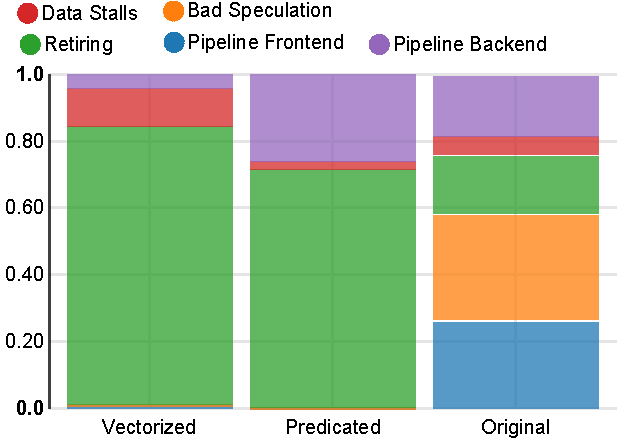
\includegraphics[width=.85\columnwidth]{Figures/damon/CostBreakdownEfficient}
  \caption{Cost breakdown of single-threaded implementations}
\vspace{-2.5ex}
  \label{fig:breakdown-efficient}
\end{figure}
\subsection*{Vectorization}
\label{sec:vectorization}
The main problem with the predicated implementation is the effort
spent on backing up data (indicated by the \emph{Pipeline Backend} bar
which includes costs for writing data in
Figure~\ref{fig:breakdown-efficient}).  The main tuning parameter for
this operation is the granularity at which data is copied. Naturally,
copying larger chunks results in more predictable code (at
compile-time as well as run-time). The extreme case for this
optimization would be copying the entire input-array, making it an
out-of-place implementation. This is not only memory intensive but
also cache-inefficient since it requires two scans of the data. The
natural solution to this problem is vectorization: small,
cache-resident chunks of the input data are copied and, subsequently,
partitioned out-of-place (see
Figure~\ref{fig:vectorized-cracking}). This has the advantage of
producing tight, CPU-efficient loops in the (expensive) partitioning
phase while allowing bulk-backups of input values.

However, the lack of control in the partitioning phase slightly
complicates things in the backup: we have to deal with overflowing
output buffers. It is, therefore, not enough to back up one vector per
side since a half-full buffer may overflow into the adjacent one. This
requires additional backup slots to ensure that the distance between
each read-cursor and the trailing write-cursor is greater than the
size of a vector. As visualized in
Figure~\ref{fig:vectorized-cracking}, three backup slots are
sufficient to maintain enough ``slack space'' for safe writing.

\subsection*{SIMD}
\label{subsec:single-threaded-simd}
Figure~\ref{fig:breakdown-efficient} indicates that more than 80\% of
the cycles of the cracking implementation are now spent retiring
(useful) instructions. This indicates that, to further improve
single-threaded performance, we have to perform more work per
instruction. This can be achieved by the use of SIMD instructions. The
AVX-2 instruction set of current Intel CPUs provides instructions to
gather values from multiple addresses into an SIMD word in a single
instruction. The opposite, i.e. scatter instructions, are, however,
only available in AVX-512 which is, currently, only supported by the
Intel Xeon Phi extension cards. We, therefore, implemented
\emph{Cracking} using AVX-2 instructions to gather the input
values. The main idea is to have one cursor per SIMD lane, gathering
values that satisfy the partitioning predicate until the word is
filled and can be flushed. We implemented all necessary operations
(comparison, cursor advancing, ...)  using 256-bit SIMD instructions
and predication.

During evaluation~(see Section~\ref{sec:results}), we found that this
algorithm generally performs worse than the previously discussed
implementations. We include the description primarily for completeness
sake.
\begin{figure}[!t]
\begin{center}
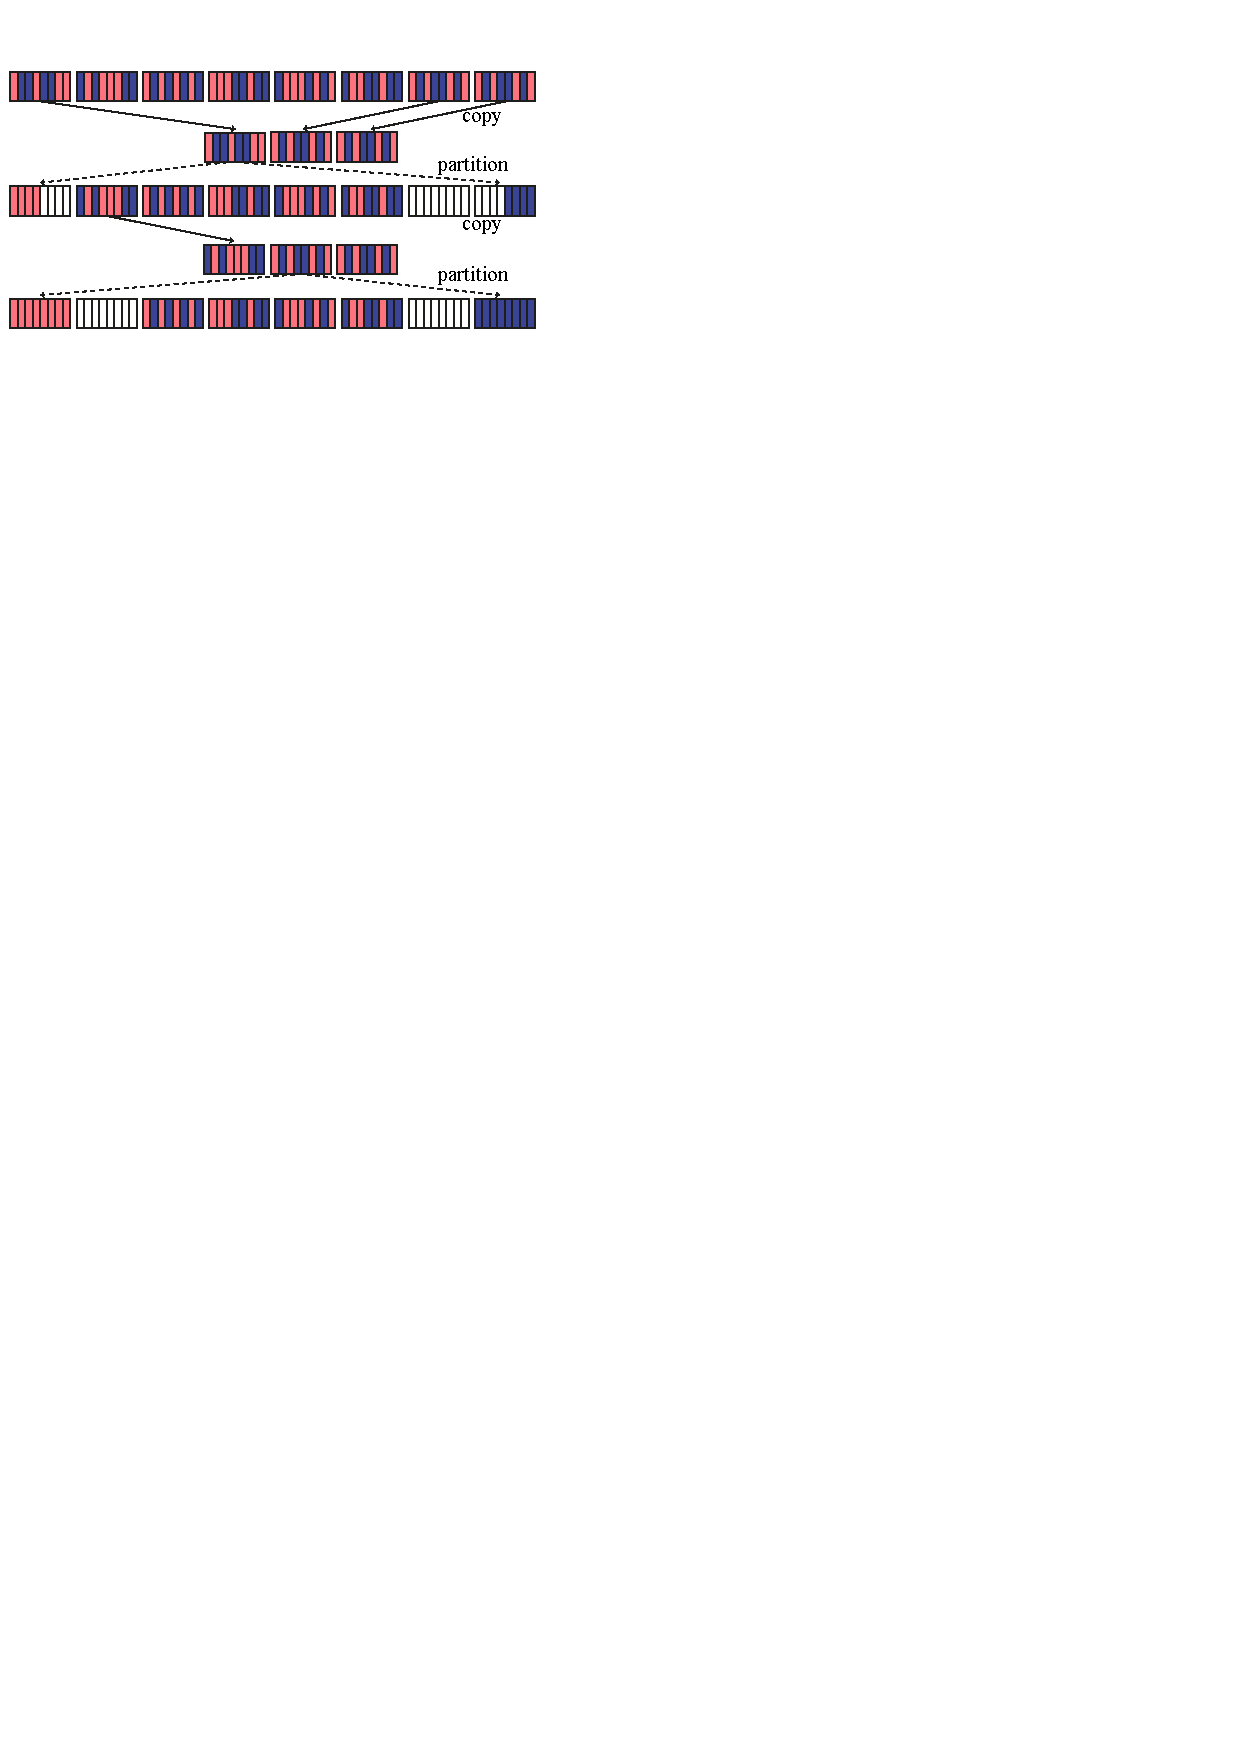
\includegraphics[trim=0cm 24.5cm 0cm 1cm,width=2.3\columnwidth]{Figures/damon/vectorized}
\vspace{0ex}
\caption{Vectorized Cracking}
\vspace{-2.5ex}
% \vspace{-0.26 in}
\label{fig:vectorized-cracking}
\end{center}
\end{figure}

\section{Parallelization}
\label{subsec:tlp}

In this section we present two \emph{Cracking} algorithms that exploit thread-level parallelism, i.e.,
first a simple partition \& merge parallel algorithm, and 
then a refined variant of the simple algorithm.

\subsection*{Partition \& Merge}
\label{subsubsec:partition-merge}

\begin{figure}[!t]
\begin{center}
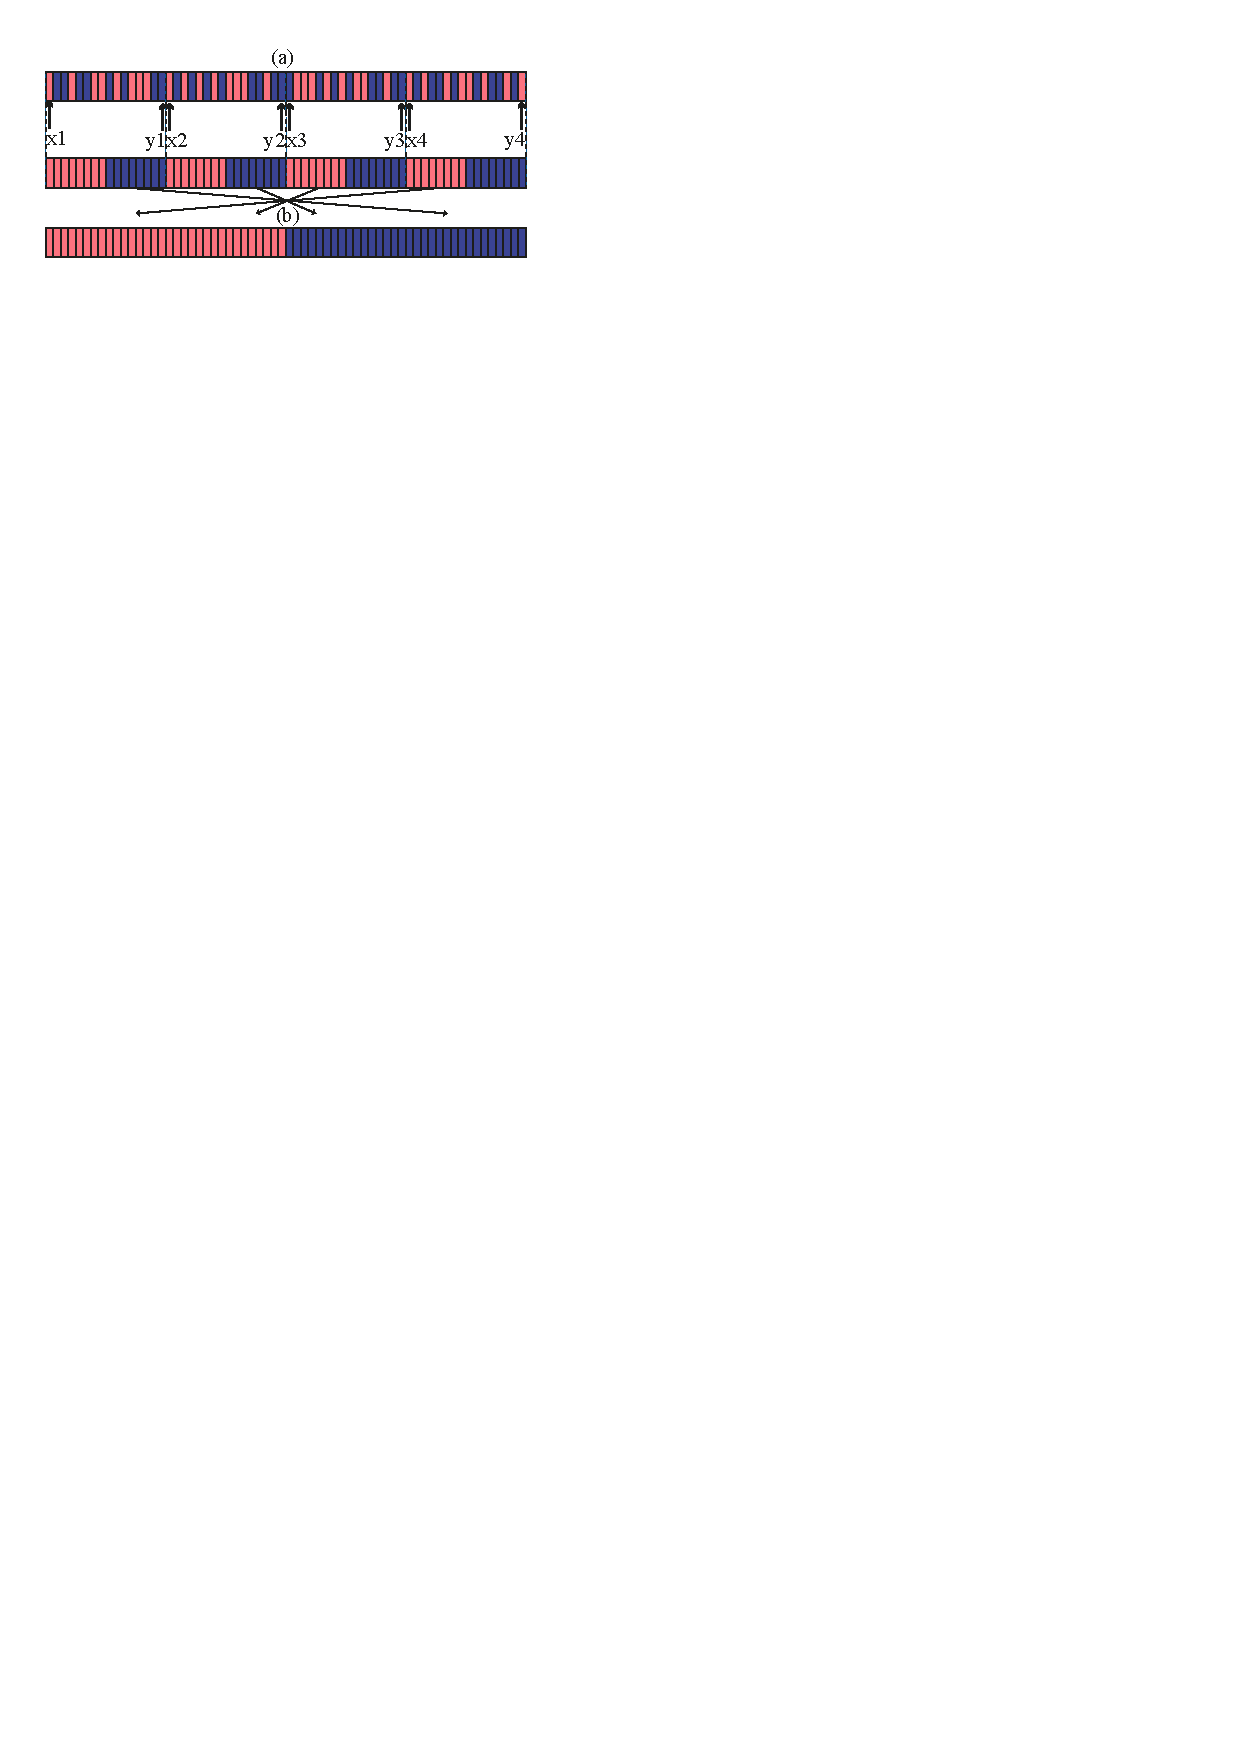
\includegraphics[trim=0.6cm 25.5cm 0cm 1cm]{Figures/damon/mcrack1}
% \vspace{-0.1 in}
\caption{Simple Partition \& Merge (multi-threaded)}
\vspace{-2.5ex}
% \vspace{-0.1 in}
\label{fig:mcrack1}
\end{center}
\end{figure}

The simple parallel \emph{Cracking} algorithm divides an
uncracked piece into $T$ consecutive partitions that are
concurrently cracked by $T$ threads.  Each thread cracks a partition by
applying the original \emph{Cracking} algorithm.  Finally, during the merge phase, a single thread swaps
wrongly located blocks of values into their final position.
Figure~\ref{fig:mcrack1} shows an instance of the simple parallel
\emph{Cracking}.  Four threads crack four partitions concurrently.
Red indicates values that are less than the pivot, while
blue indicates values that are greater than the pivot.  
After cracking all partitions, the merge phase takes place, i.e., a single thread relocates blocks of elements to the correct positions, resulting in the final cracked piece shown in Figure~\ref{fig:mcrack1}(b).
During the merge phase the relocation of data causes many cache misses, which can be avoided with the refined partition \& merge \emph{Cracking} described in the following subsection.

\subsection*{Refined Partition \& Merge}
\label{subsubsec:refined-partition-merge}

\begin{figure}[!t]
\begin{center}
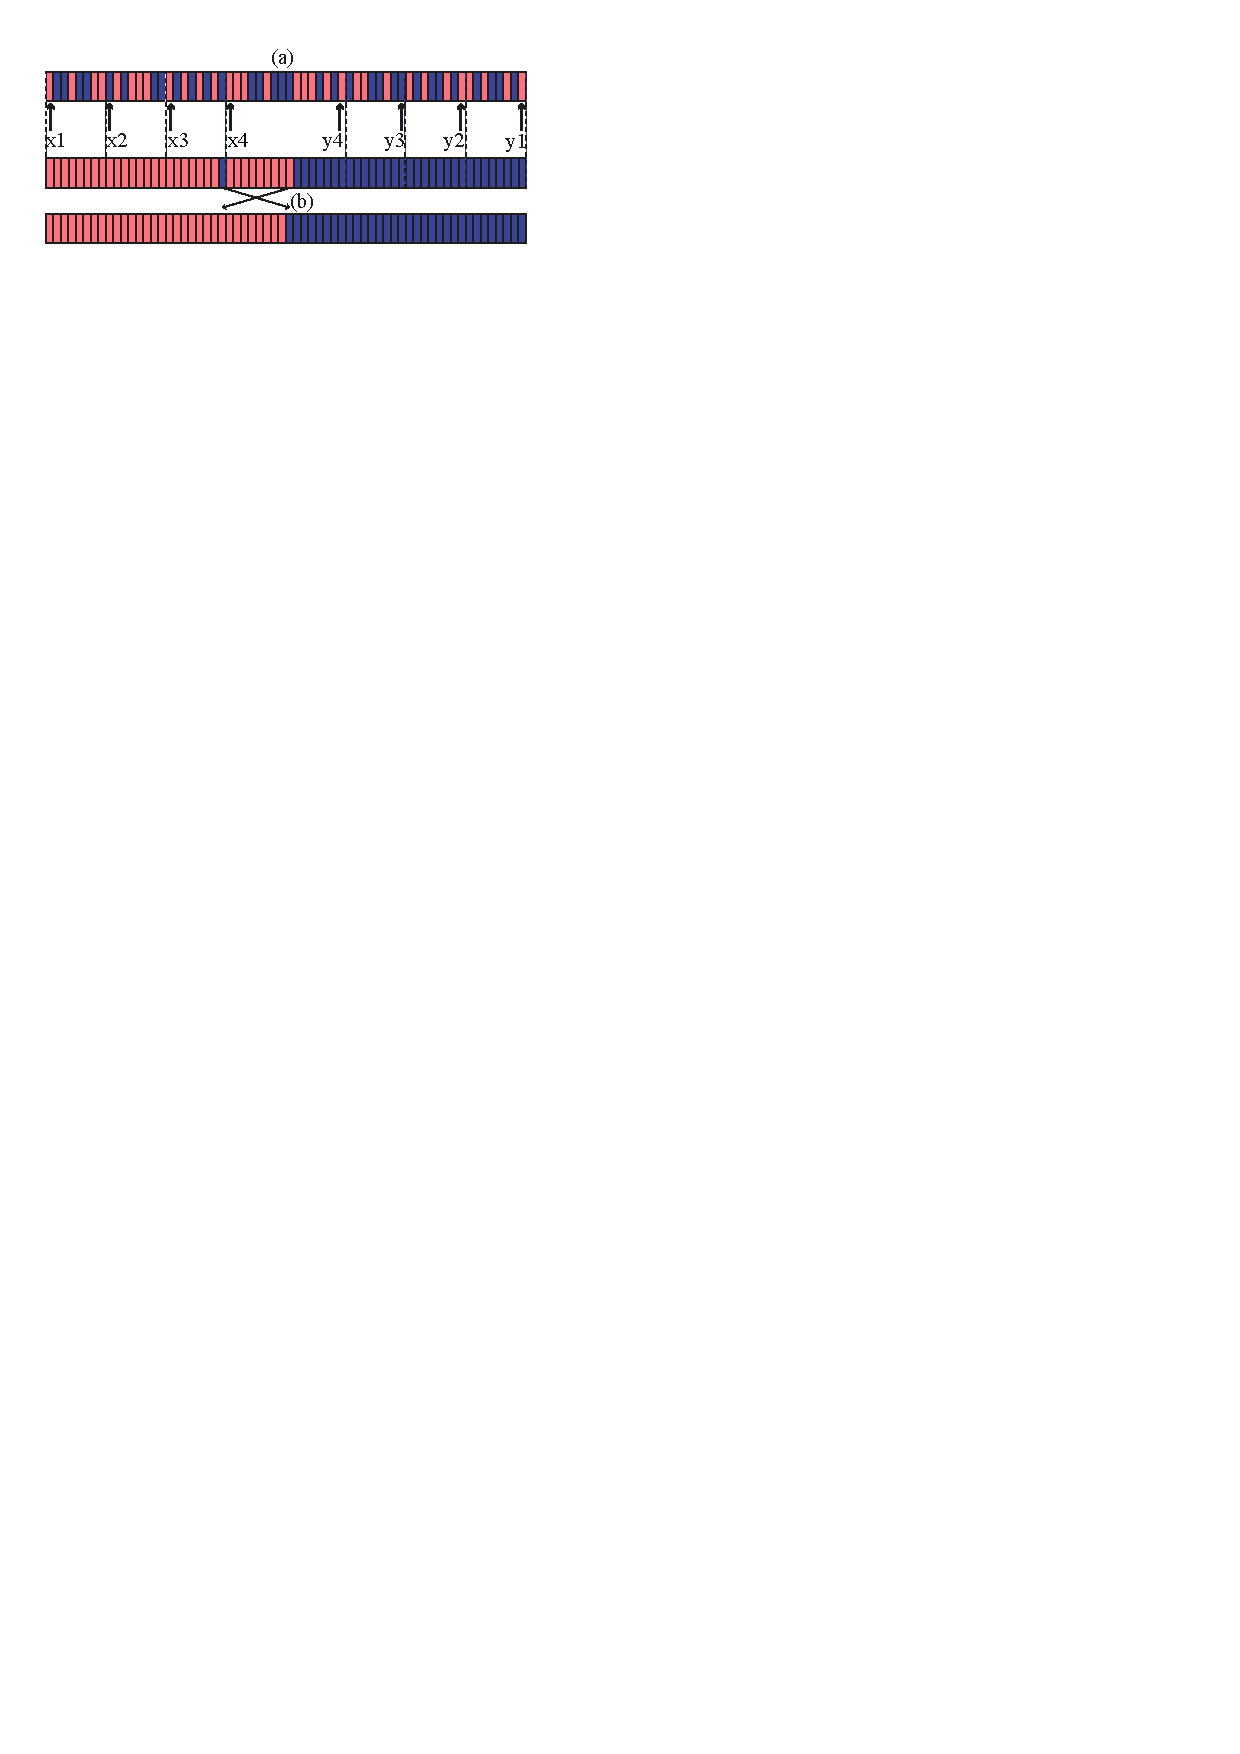
\includegraphics[trim=0.6cm 25.7cm 0cm 1cm]{Figures/damon/mcrack2}
% \vspace{-0.2 in}
\caption{Refined Partition \& Merge (multi-threaded)}
\vspace{-2.5ex}
% \vspace{-0.4 in}
\label{fig:mcrack2}
\end{center}
\end{figure}
The refined partition \& merge \emph{Cracking} algorithm divides the uncracked
piece into $T$ partitions.  
The center partition is consecutive with
size $S=\#elements/\#threads$, while the remaining $T-1$ partitions consist of two disjoint
pieces that are arranged concentrically around the center partition.
Assuming the selectivity is known and it is expressed as a fraction of 1, the size of the left piece equals to $S*selectivity$, while the size of the right piece equals to $S*(1-selectivity)$.
For instance, in Figure~\ref{fig:mcrack2}(a), the size of the disjoint pieces is equal, since the selectivity is 0.5 (50\%).
As in the simple partition \& merge \emph{Cracking}, $T$ threads
crack the $T$ partitions concurrently applying the original \emph{Cracking} algorithm.  
The thread that cracks the center (consecutive) partition, swaps values within this partition.
Each thread that cracks two disjoint pieces swaps wrongly located values between the
two pieces.  For example, in Figure~\ref{fig:mcrack2}(a) one thread exchanges values between the first and the last piece.
Finally, a single thread (as in the simple parallel algorithm) locates wrongly-located blocks to the correct positions.

Although the refined algorithm swaps values that are in longer
distance compared to the simple algorithm, it moves less data during
the merge phase, because more data is already in the correct position.
For instance, in Figure~\ref{fig:mcrack2} only two values are located in wrong positions, while in Figure~\ref{fig:mcrack1}, we relocate 6 blocks of 8 values each.
Both parallel algorithms make $O(n)$ comparisons/exchanges during the partitioning phase.
However, the merging cost is significantly lower for the refined partition \& merge \emph{Cracking} algorithm.  


\subsection*{CPU Efficiency \& Parallelization}

In principle, the single-threaded CPU efficiency improvements as presented in
Section~\ref{sec:cracking-algorithms} are orthogonal to the thread-level
parallelism presented above. Consequently, we can combine both techniques,
hoping to accumulate their benefits. We focus on vectorization as this proved
to yield better single-threaded CPU efficiency than predication or SIMD
(cf., Sections~\ref{sec:cracking-algorithms} and \ref{sec:results}).

Vectorization of the simple partition \& merge \emph{Cracking} algorithm is
straight-forward.  We simply have each thread perform vectorized
\emph{Cracking} instead of original \emph{Cracking} on its contiguous
partition.  With the refined partition \& merge \emph{Cracking} algorithm,
we need to additionally handle the case that, in case of skewed data, one of
the two write cursors exceeds its partition half, and thus needs to
``fast-forward'' (or ``jump'') to the other half to continue.

